\fancyhead[LO]{{\scriptsize {\FA \ }我们最幸福 {\FA } 酒瓶当点滴}}%奇數頁眉的左邊
\fancyhead[RO]{{\tiny{\textcolor{Gray}{\FA \ }}}\thepage}
\fancyhead[LE]{{\tiny{\textcolor{Gray}{\FA \ }}}\thepage}
\fancyhead[RE]{{\scriptsize {\FA \ }我们最幸福 {\FA } 酒瓶当点滴}}%偶數頁眉的右邊
\fancyfoot[LE,RO]{}
\fancyfoot[LO,CE]{}
\fancyfoot[CO,RE]{}
\chapter*{07 {\FA } 酒瓶当点滴}
\addcontentsline{toc}{chapter}{\hspace{5mm}07 \textbf{>}\ \ 酒瓶当点滴}
\vspace{15mm}
\begin{flushright}
	\textcolor{PinYinColor}{\EN \huge{Two Beer Bottles\\
		for Your IV\\
	\ \\}}
\end{flushright}

\begin{figure}[!htbp]
	\centering
	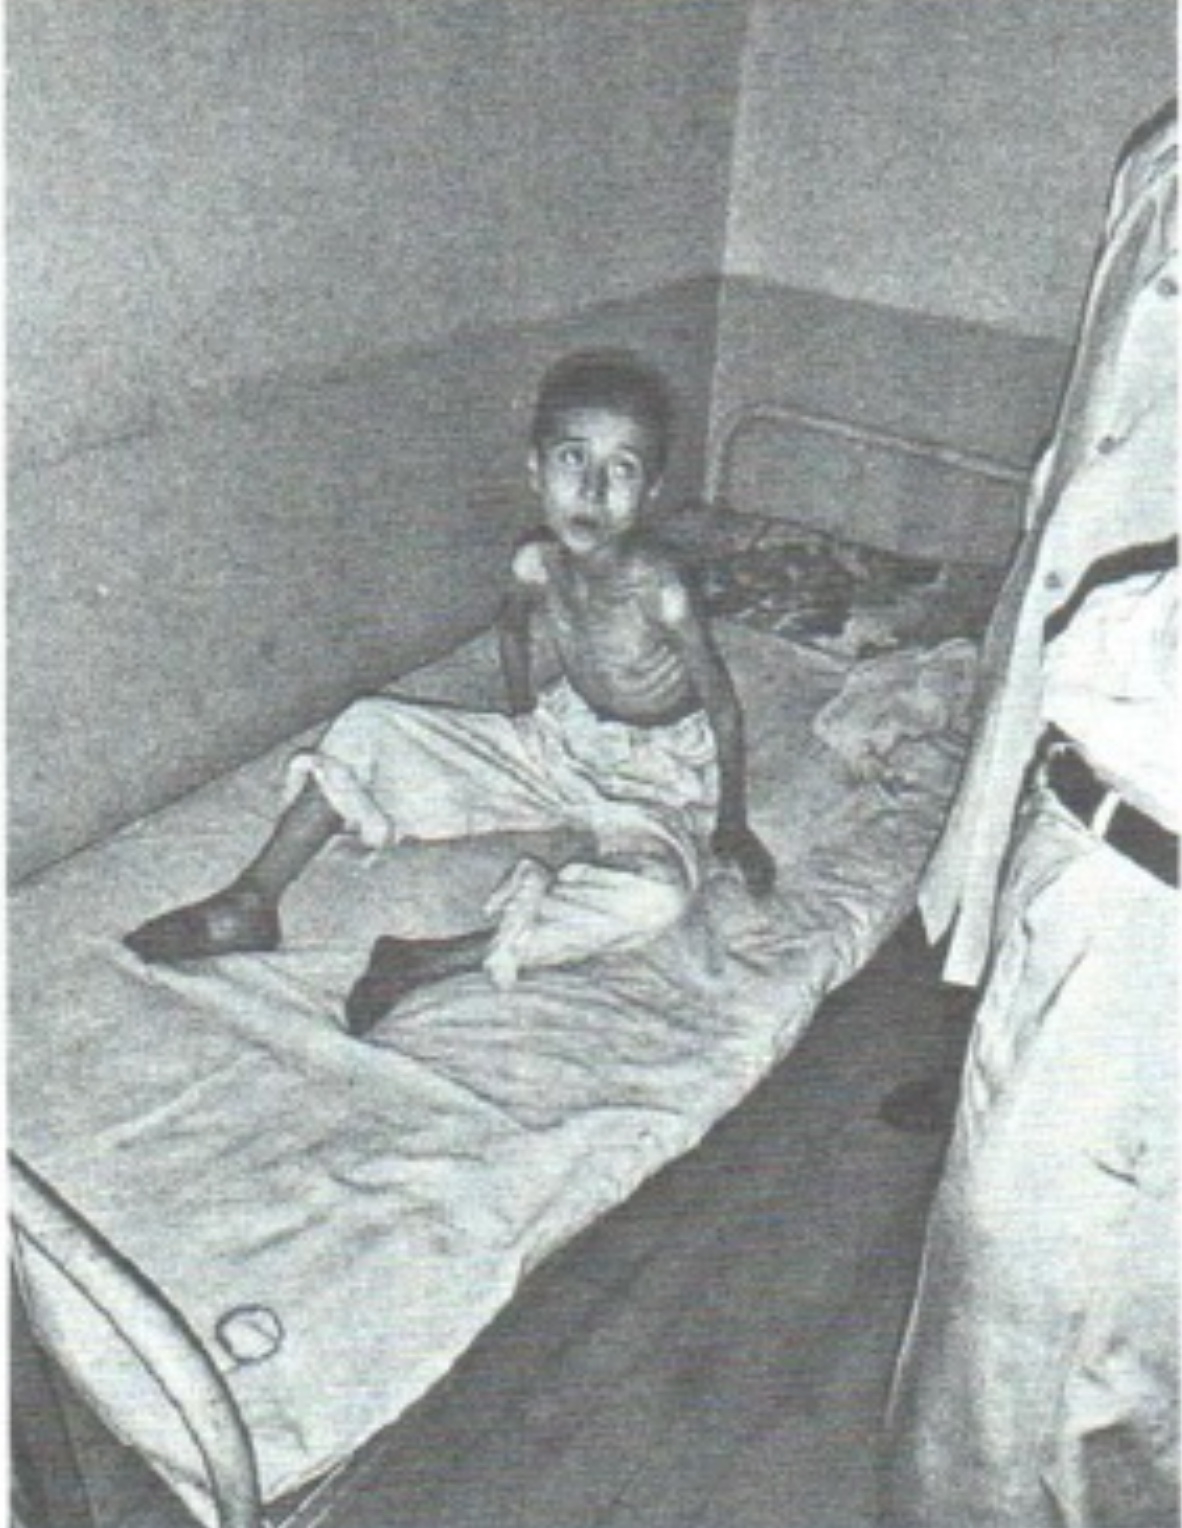
\includegraphics[width=6cm]{./Chapters/Images/07.jpg}
	\caption*{咸兴医院里的男孩}
\end{figure}

\ifnum\theparacolNo=2
	\begin{multicols}{\theparacolNo}
\fi
金日成去世时,清津已经没有汽油开动屈指可数的那几台救护车,病人必须靠人背着或是用木头推车送到医院。金智恩在一家小的地区医院工作,因为这家医院离浦港广场最近──走路大约只要15分钟,所以那些在铜像前推挤中受伤或晕倒的人全都被送来了,让这家原本就很小的医院更是显得人满为患。金属病床上都躺满了病人,一个小病房里挤了五张床,还有更多人坐在木头长椅上或躺在昏暗的走廊上候诊。医院内白天很少开灯,因为电全被用于不分昼夜的照亮金日成铜像。由于伤寒疫情爆发,这个夏天本就忙碌异常。在儿科,父母带着病怏怏的孩子来看医生,这些孩子都是在骄阳下啼哭而导致了严重的脱水,有些人甚至出现痉挛现象。通常金医师的工作时间是从早上7:30到晚上8点。不过这些日子,除了抽空到铜像前表达哀思,她几乎整天都待在医院。尽管如此,她从未抱怨工作时间过长。金医师非常看重自己的行医信约。何况辛苦工作也能让她暂时忘却自己早已亮起红灯的个人生活。\\

28岁的金医生是这家医院最年轻的医生,也是个子最小的。她穿上鞋也不过150公分,勉强能够高过她的小病人,体重也不到45公斤。金医师有着像弓一样略弯的嘴唇和心形脸蛋,给人纤细柔弱的感觉。或许是为了避免这点,她总是摆出一副严肃的态度,而且她的同事,尤其是男同事,很快就明白不能小觑她。虽然认为金医生不容易相处,但他们都认为她是个好医生。她总是第一个志愿承担那些无薪的额外排班。下班后,金医生还要到劳动党书记办公室工作。就跟北朝鲜其它机构一样,医院也设有党委书记。党委书记的工作是确保工作场所意识形态的正确,与挑选适当的入党人选。虽然医院里大概每四名医生才有一名有机会获准入党,金医生却很自信自己会被选中。其中一个理由是女性比较容易获准入党,因为女性绝大多数不喝酒,而且一般来说比较守规矩。其次是金医生自律且不苟言笑的性格,未来也会是个尽心尽力的党员。她对北朝鲜政府的奉献与热爱无疑是真诚的,因为她自小就受到父亲的熏陶。\\

在朝鲜和中国边境──图们江、鸭绿江上,几个世纪历经来来回回的迁徙,因此满洲有着大量的朝鲜族人口。金医生的父亲就是在出生在中国靠近朝鲜边境的一个说朝鲜语的村子里。在60年代早期,还是个年轻人的时候,为了逃离毛发动的灾难性的大跃进及引发的导致数百万人死亡的大饥荒,他来到了北朝鲜。金医生的父亲认定是金日成而不是毛,才真正代表着共产主义,是能给像他一样的工人阶级以真正平等及公正的对待。他仅仅是一个建筑工人,只读过6年书,但是他的聪明才智,全心奉献都被北朝鲜所认同,他甚至还被劳动党接纳为党员。他在所工作的建筑队担任党委书记直到几年前的轻度中风后才从岗位上退休。因为没有儿子,他所有的希望都寄托在女儿身上,希望女儿能够替他继续为党、为祖国奉献一生。\\

未来的金医生对所担负的责任也是满怀激情。在7岁的时候,她光荣的加入少年先锋队,脖子上戴上少先队标志性的红领巾。在13岁的时候,她进一步加入社会主义青年团,并且自豪万分的佩戴上金日成像章。加入青年团几乎是每个北朝鲜人必经的仪式,但是对于一个13-14岁或者15岁的孩子来说,加入青年团要靠个人的操行及学习成绩。还早在小学低年级的时候,金智恩就表现出比其它孩子成熟。\\

她写的一手漂亮的好字,上课也总是第一个举手回答老师的提问,学习成绩也总是名列前茅。还在学校读书的时候,她就被特别选拔进去医学院学习,尽管她曾经梦想当个教师或者记者。然而作为一个建筑工人的女儿能被选择成为未来的医生,也是莫大的荣誉了。\\

还在16岁的时候,她就进入清津医学院,她的同学们都比她大2岁,而且2/3是女生。在完成7年的学习后,她开始在学校的附属医院,也是咸镜北道最富盛名的道第二人民医院的实习。那时候,她看上去仍然像个只有十几岁的青少年。当地人把这个医院叫做“捷克医院”,因为早在60年代,朝鲜还是社会主义大家庭中的一员时,有一队来自捷克斯洛伐克的医生带着X光机和育婴箱在这里施诊。现在虽然捷克的医生早已离开,大部分的医疗设备都被塑料带封存了起来,但是医院仍然保留着欧洲医院的名声。实习期过后,金医生作为正式医生被分配到一个小医院,这个医院服务于浦港区,她就住在这一区。\\

金医生早上7:30就要到单位报到。按规定,她每天需要工作12小时,看至少32名病人。通常上午她会在医院,而下午则会随医疗小组出诊。她穿白大褂,头戴可以罩住头发的白帽子,使得她看上去像个做快餐的厨师。她总是随身带个很重的医疗包,里面装着听诊器、注射器、绷带、消化药片、抗生素等等。作为3人医疗小组的成员,她要走访学校小区。朝鲜每个小区都有卫生室,同人民班设在一起。\\

“医生出诊!医生出诊。”这样的喊声回荡在小区里。之后,人们就会在小区卫生室前排起队,大人带着哭闹的孩子排成一队,准备让医生处理手上的伤口,或者身上出了几个星期的疹子。\\

北朝鲜的医生被期望无私地为人民服务。由于缺乏X光机,他们通常只能使用简单的X光透视机,让病人曝露于高度辐射下;不少老医生也因此落下白内障。需要的时候,医生不仅要捐血,还要捐出小块的皮肤移植给烧伤病人。金医生因为身高体重远低于平均值,得以免除这最后一项义务,但她仍然要到山上采摘药草。\\

亲自调制药品也是北朝鲜医生的要务,住在温暖气候地区的医生还要自己种植棉花来纺制绷带。医生全都得外出采集药草。金医生的工作单位尽可能在春秋两季各腾出一个月的时间让医生去采集药草。这段期间,他们睡在荒郊野外,几天才洗一次澡。每人都得采集到规定的数量,然后将采到的药草运回医院的药剂室,接受秤重。如果重量不足,还得继续去采。他们通常要深入山区人迹罕至之处,因为比较容易到达的地方早已被想卖药草或留作自用的人们给采光了。其中最抢手的是芍药根,能用来放松肌肉,治疗神经疾病。野山药可调节女性月经周期,蒲公英有助消化,姜可以防止恶心。苍朮属植物也是一种颇受欢迎的中药,能增强免疫力,没有抗生素的时候就得靠它了。\\

多年来,北朝鲜医院一直采用草药疗法结合以西药。医师不用止痛药,而用拔罐──一种让有吸力的小杯刺激人体特定部位以促进全身血液循环的方法。另一种方法也是源自于中医,就是用艾草针灸患病部位。由于缺乏麻药,对一些简单的手术如切除阑尾,医生就用针灸代替。“有效的时候会很有效”,多年后,金医生这么跟我说。没效的时候呢?病人会被绑在手术台上,以免他们乱动。多数时候,北朝鲜人在接受治疗时都很能忍痛。“他们才不像南韩人,稍微有点小病就喊得震天价响”,金医生说。\\

尽管有很多缺点,北朝鲜的公共卫生系统还是给予人民远优于共产党时期之前的医疗服务。这种享受“全面性的免费医疗服务……改善劳动人民健康”的权利,实际上明文规定在北朝鲜宪法上。金医生对自己身为这个医疗体系的一员也颇为自豪,也对自己能提供病人医疗服务感到高兴。但到了90年代初期,北朝鲜医疗体系的弊端日益凸显。许多医疗设备不是过时就是不堪使用,原本制造这些机器的社会主义集团国家的工厂现如今都已私营化了,因此也得不到设备的配件。清津的制药厂因为缺乏原料与电力而减产。北朝鲜也没有资金从国外进口药品。金医生巡诊时提的袋子越来越轻,以至于到最后里面除了听诊器什么都没有了。她只能帮病人开处方,希望他们有亲戚朋友在中国或日本,或是用私藏的钱从黑市买到药品。\\

1993年,金医生首次与医院领导层发生严重冲突,令她心灰意冷。当时她负责诊疗一名27岁的男子,这名男子被判以经济罪──也就是说他曾经从事私人买卖。他被判7年有期徒刑,在服刑满3年后,从监狱转到了医院。这人被打的全身是淤青而且严重营养不良,瘦得连肋骨都清晰可见。他还患有急性支气管炎。金医生想给他打抗生素,却遭到领导拒绝。\\

“他是罪犯,我们应该把抗生素留给其它人”,上级告诉金医生。\\

金医生愤怒了。“他已经被送到医院来了,病人就是病人,我们可以救他。他没有抗生素的话,可能连命都保不住”,她严正地反驳。\\

她执拗的一面在这件事上表露无遗。金医生并不善罢干休,为此事她同领导一连争论了数日。最终,垂死的年轻人还是没有治疗就出院了。金医生每天到他家两次,但这名病人的病情却日益严重,意志也越来越消沉。他嚷着:“我不应该继续活下去。”不久就自杀了。金医生深信自己和医院要为他的死负责。她和上级之间的紧张的关系也一直持续着,于是她主动申请调到儿科,她认为那里的情况不会这么政治化。\\

于此同时,金医生的个人生活也出了问题。不像事业上的成功,她的爱情生活一点也不美满;她工作狂加完美主义的风格,使得男人们对她都敬而远之。在正式参加工作后1年,从大学时代就开始约会的男友和她分手了。此事对她打击巨大。她求朋友帮她介绍了一个人,在第二次约会后就同他订了婚。她丈夫同她一样年纪──26岁──但是由于在军队服役,此时还只是个大学一年级新生。由于她已经工作了,她想他们可以依靠她的工资直到丈夫毕业。\\

“你会伤了他的自尊心。”金医生的母亲担心的说。一个女医生嫁个一个大学生?“男人不喜欢他们的妻子赚的比他们多。”\\

在结婚的当晚,金医生意识到她犯下了个多么可怕的错误,但是她很快就怀孕了,因此也没有机会逃离。几个月后她生下了孩子,在给年幼的儿子哺乳完之后,她搬出了丈夫家,回到了自己父母家。按照朝鲜传统,孩子由她的公婆照顾;如果离婚的话,孩子的监护权也在父亲一边。\\

如果赚的多是她婚姻不幸的罪魁祸首的话,那么令人颇为尴尬的是,她的薪水最终却消失了。她曾经能赚186朝元一个月,按照官方汇率大概值80美元,是一般普通工人的3倍。用这些钱,她可以养活丈夫,自己的父母,甚至还能帮衬一个已经出嫁的妹妹。随着薪水消失的还有食物配给。在此期间,她发现自己不得不去集体农庄的果园去偷梨子,在乡下去搜集吃的。她也时不时的接受病人的礼物──一袋面条或几个玉米棒,这使得她觉得非常尴尬及不舒服。金医生知道其它医生收取贿赂以换取原本免费的医疗服务;她决定不与他们同流合污。但是回过头来,她也饥肠辘辘。\\

在28岁的时候,她早年的美好憧憬慢慢都变成失望。她离婚了,同父母住。她失去了孩子的监护权。她现在比以前更加努力的工作,然而得到的回报却比以前还要少。她又饥又累,贫穷而且找不到真爱。\\

这就是金医生在金日成死的前1年的不幸处境。\\

与大多数北朝鲜人一样,金医生是从中午的特别广播中得知金日成的死讯。当时她才护送完一名伤寒病人到一间特殊诊所,刚刚回到医院。进到医院大厅,就看到医生、职员与病人全在全院唯一一台电视机前面哭泣。\\

金医生花了40分钟才走回自己位于市体育场后面的公寓,她的眼睛噙满泪水,几乎看不清自己蹒跚在人行道上的双足。父亲在家睡觉。听到她的脚步声,于是坐了起来。\\

“怎么了?你的病人过世了吗?”他惊慌地问。他知道自己的女儿对病人投入的感情有多么深。\\

金医生倒在父亲怀里。她从来没有哭得如此伤心过,即使是在男友抛弃了她,婚姻破裂孩子被带走,还是父亲中风的时候。这些全是人生可预期的挫折。即使金医生是一名医生,受过高等教育,了解人的自然规律,也深知人不免一死,但她从来没想过这样的事会发生在金日成身上。\\

她同事的感受也差不多。当他们在医院昏暗的走廊上彻夜工作时,会交换自己听到的小道消息。其中一种说法是,金日成是被美国的军火贩子暗杀的,因为他们想破坏即将来临的南北高峰会,届时金日成会跟南韩总统金泳三会面──北朝鲜宣传政策中反复出现的一点就是美国蓄意让朝鲜半岛分裂。\\

金日成刚去世的那几天,金医生过着浑浑噩噩的日子。由于处于震惊与睡眠不足之下,她隔了好一阵子才发现,自己家里也早已危机重重。她的父亲自从因病退休之后就陷入忧郁,伟大领袖的死对他更是个打击。他躺在床上,拒绝进食。\\

“如果像金日成这么伟大的人都会死,那像我这种一无是处的人又何必活着浪费粮食?”他哭道。\\

金医生试着跟她的父亲讲道理。先是好言相劝,然后提高音量,最后连威胁也用上了。\\

“如果你不吃,我也不吃。我们一起死好了。”她这么说。她的母亲也威胁要绝食。金医生还把医院的党委书记找来一起劝他。她也试着用静脉注射的方式让父亲维持体力。\\

金医师的父亲开始呓语。他一会儿赞美金日成,一会儿又辱骂他。一天他说自己是如此敬爱领袖,没有领袖他活不下去,另一天他又低声说金日成的死清楚的证明了北朝鲜的体制完全失败。他要女儿从医院带些纸回来,勉强撑起身子,潦草地写了张便条:\\

身为劳动党党员,我最后的任务就是让我的长女继续我的工作。请指导她,让她成为优秀而忠诚的党员。\\

他把信交给金医生,要她转交给医院的党委书记。然后他又拿了一张纸,在上面胡乱画了一个看似相当复杂的金字塔,每个塔阶标示着姓名与数字,那个图怎么看都像是疯子的涂鸦。金医生以为父亲神智不清了。\\

他示意金医生坐到他的身旁。他身体已经虚弱得只能轻声说话。\\

“这是我们家在中国的亲戚。他们会帮你。”\\

那是一张族谱。金医师感到震惊。难不成父亲是在暗示她离开祖国,到中国去?这是逃离中国后,亲自跪着教导她读书写字,对金日成忠诚无比的父亲会说的话吗?他会是叛徒吗?金医生第一个反应是撕碎它,但她无法毁掉父亲的遗言。于是她拿出一个收藏纪念品的小铁盒,上面有锁与钥匙,这是她少女时期留下来的东西。\\

她把父亲的草图折好,锁进箱子里。\\

金日成安厝于一处地下陵寝,他的遗体在经过防腐处理后公开陈列,这是1924年列宁(Vladimir Lenin)死后共产党的传统。北朝鲜政府举办了为期两天\footnote{金日成葬礼为7月19日与20日。}的隆重葬礼。平壤广播电台报导有200万人参加了这场仪式,金日成的灵柩放在凯迪拉克车顶上巡回整座城市,后头跟着踢正步的士兵、军乐队、以及架有领袖肖像与花叶装饰的加长型礼车车队。百辆车组成的车队行列从金日成广场出发,行经金日成大学与市中心23米高的金日成铜像\footnote{该铜像是北韩最大的金日成铜像。},最后停在革命门前,这是巴黎凯旋门的仿制品,只是更为巨大。次日有一场纪念仪式。正午12时,全国各地警报声响起,车辆与船只鸣按喇叭,每个人立正默哀3分钟。国丧期间终于结束。该是国家返回正轨的时候了。\\

金医生有许多机会藉由工作来忘记悲伤。她的父亲在金日成葬礼后的一个星期去世,所以她晚上也不想回家,宁可更长时间的工作。热浪尚未结束,始于夏天的伤寒现在成了席卷各地的重大疫情。因为排水系统不佳,清津市很容易爆发疫情。排水系统是在朝鲜战争后仓促重建的,未处理过的粪便被冲入妇女用以洗衣的河川。随着电力断断续续,自来水也不太稳定。通常早上与下午会有1小时的水电。人们在家里用大桶子储水\footnote{在朝鲜几乎没有人有浴缸。},而这些水桶就成了细菌温床。没有人有肥皂。伤寒可以用抗生素轻易地加以治愈,但到了1994年,北朝鲜却几乎得不得这种药品。\\

1994年的炎夏之后,迎来了罕见的寒冬,山区气温骤降至-35度。来年夏天出现暴雨,洪水淹没了农田。这让北朝鲜政府有了不失面子的借口,首次公开承认国内出现粮食短缺。1995年9月,联合国赈灾小组获准进入北朝鲜,他们得知水灾所造成的损失已达150亿美元,520万人受灾;96348栋民宅被毁,50万人无家可归;减产190万吨的农作物。\\

在儿科病房,金医生则注意到她的病人出现一些奇怪的症状。在她治疗的孩子当中,凡是80年代晚期到90代早期出生的,体格都小的惊人,甚至比金医生自己读小学时的个子还小,她当时是班上最矮小的学生。这些孩子的前臂瘦到金医师只需要用自己的食指与大姆指就能轻易圈住。他们的肌肉软弱无力。这是肌肉耗损的症状,也就是身体在饥饿状态下会吃掉自身的肌肉组织。这些孩子因便秘而来看诊时,症状非常严重,以至于他们痛得蜷缩着身体,痛苦的嚎叫。\\

问题出在食物上。粮食短缺使得家庭主妇开始采集杂草与野草加到汤里面,营造出一种蔬菜的假象。玉米逐渐取代大米成为主食,而且还在玉米里参入玉米叶、玉米壳、玉米茎与玉米芯使得玉米饭煮的更多一些。大人还撑得住,孩子稚嫩的胃可受不了。在医院里,医生们一起讨论这个问题,最后他们决定给这些母亲一个烹煮上的建议。“如果你们要煮野草或树皮,就必须把这些东西磨得很细,然后煮久、煮软一点,这样比较容易吃”,金医生告诉她们。\\

年纪稍大些的孩子与成人则是出现另一种奇怪的新症状。病人的双手和沿着锁骨一圈长出发亮的疹子,长在锁骨附近的,感觉就像戴了项链,要是长在眼睛周围,看起来如同戴了眼镜。这种症状有时被称为“眼镜病”。事实上这是糙皮症\footnote{玉蜀黍疹。},主要是饮食中缺乏烟碱酸所引起,通常发生在只吃玉米的人身上。\\

常常有因为小感冒、咳嗽或腹泻而来看诊的孩子在很短的时间内突然死亡。贫乏的饮食降低了他们的抵抗力。就算医院有抗生素,他们虚弱的身体也吃不消。婴儿骨瘦如柴,他们的母亲自己也营养不良,无法分泌足够的乳汁。在这里,婴儿配方奶粉闻所未闻,连普通牛奶都很罕见。过去,奶水不够的母亲会用稀释的粥来喂孩子,现在她们连米也买不起。\\

另外还有一些孩子完全没有可诊断的症状,只是抑郁。他们看起来脸色苍白或者有点发青,皮肤粗糙缺乏弹性。有时候肚子会鼓胀,但有时候又没有。\\

“我不知道我的孩子得了什么病,我就是无法让他停止哭闹”,母亲们这么对金医生说。\\

她同情地点点头。她了解这个状况,却无法把话说出口。在没有粮食的状况下,你要如何告诉一名母亲,她的孩子需要的只是多吃一点?\\

金医生会写下便笺,让这些孩子住院,虽然明知自己根本无法治疗他们。医院也没有食物。当她巡房时,经过儿科病房,孩子们的目光跟着她的身影。即使当她转身时,她也能感觉到孩子们的眼睛盯着她的白袍,想着她是否能解除他们的痛苦,然而很快就明白她也无能为力。\\

“他们看着我的眼神充满指责。即使是四岁的孩子也知道自己快死了,而我一点忙也帮不上。”多年后,金医生这么对我说。“我能做的只是事后跟着母亲们对着他们的尸体痛哭。”\\

金医生从医的时间还没有长到已经在自己与病人之间筑起一道保护墙。孩子的痛苦就是她的痛苦。几年后,当我问她还记不记得一些在她注视下死亡的孩子时,她斩钉截铁地回答:“每个孩子我都记得。”\\

几年过去了,医院能提供的治疗越来越少。地下室的火炉将煤炭烧尽之后,变成一个摆设,于是医院的暖气停了。当停水的时候,也无法适当地拖地。即使在白天,院内也是一片阴暗,医生只能站在窗边写报告。病人必须自备食物与毛毯。由于绷带稀少,病人会剪下被单权充绷带。虽然医院仍然可以进行静脉输液,但他们没有瓶子来装这些输液。病人必须自己带瓶子来,通常是用清津最受欢迎的“乐园”啤酒()Rakwon)的空瓶。\\

“如果他们带一个空瓶,就可以吊一瓶点滴。带两个空瓶,就可以吊两瓶点滴。”金医生说。“这种事很难堪,令人难以启齿,但我们就是这样做的。”\\

最后,医院人去楼空。人们不再带亲人去看病。何必这么麻烦呢?\\

金日成的死实际上并未对北朝鲜造成多大改变。金正日在他父亲去世前10年已逐渐掌握权力。经济不可避免的崩溃是经年累月的结果,其病根始于北朝鲜经济缺乏效率。但北朝鲜的伟大领袖挑了一个非常合适的时辰离开人世,往后数年的灾难也不至于使他毕生的事迹蒙尘。要是金日成多活几年,今日北朝鲜人将不会以怀旧的心情回顾在他统治期间曾拥有过的相对富足的生活。他去世之际,刚好也是共产主义美梦破灭之时。\\

到了1995年,北朝鲜的经济就跟它的伟大领导人的尸体一样冰冷如石。国民人均收入直线下降,从1991年的2460美元,陡降到1995年的719美元。北朝鲜的商品出口从20亿美元掉到8亿美元。经济的崩溃具有一种有机性,彷佛一个生命体正缓慢丧失功能,走向死亡。\\

在清津,沿海矗立的巨大的工厂像一道生锈的墙,烟囱整齐得像是监狱的铁杆。烟囱是最可靠的指标。多数时候,工厂锅炉只会喷出几阵烟,你可以清楚数出喷烟次数──一阵,两阵,顶多三阵──然后看着这城市的心跳慢慢消失。工厂大门紧闭,上头缠绕着链条和挂锁──当然了,如果早已把机械拆散、运走的小偷还没把锁也偷走的话。\\

工业区北边,海浪轻拍着空荡荡的港口码头。以往固定来载运钢板的日本和苏联货船都不见了,现在只剩下北朝鲜一些生锈的渔船。宣告着21世纪的太阳──金正日的几个大字高耸在港口上方的峭壁上,但连这几个字好像也跟周围的景观同朽了。沿路宣传告示上的红色字迹已多年未重新上漆,褪成了黯淡的粉红色。\\

清津曾是北朝鲜污染最严重的城市,现在有了一种崭新的美,荒凉又寂静。在秋冬这两个东北亚的干燥时节,这里的天空清新而湛蓝。来自钢铁厂刺鼻硫黄味已经消失,人们再次嗅到海水的气味。夏天,蜀葵悄悄从侧方爬上了水泥墙。连垃圾都不见了。这并不是说北韩以前有很多垃圾──东西都不够了,哪来的垃圾呢──但既然经济活动全然停止,文明生活的沉积物自然也随之消失。没有塑料袋或糖果包装纸随风飘荡,港湾里也没有漂浮着的汽水罐。如果有人在人行道上踩熄一根烟,就会有另一个人去捡,把香烟拨开,抽出里面仅余的几根烟丝,用报纸再次卷起。\\
\ifnum\theparacolNo=2
	\end{multicols}
\fi